\begin{figure}[H]
    \centering
    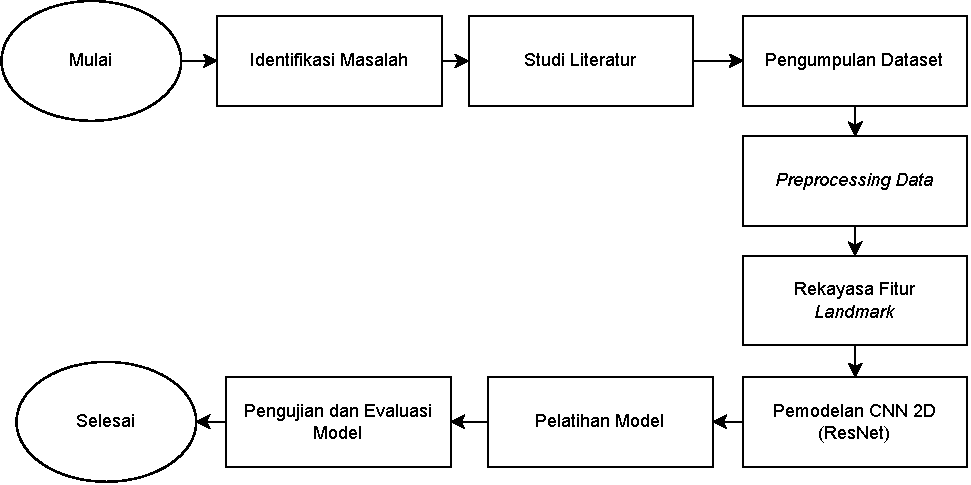
\includegraphics[width=0.9\textwidth]{figure/alur_penelitian.pdf}
    \caption{Alur Penelitian}
    \label{fig:alur-penelitian}
\end{figure}

Penelitian ini dilaksanakan menggunakan pendekatan eksperimental dengan tahapan yang disusun secara sistematis. 
Lokasi perekaman direncanakan berada pada ruang tertutup dengan pencahayaan yang stabil untuk memastikan kualitas visual yang konsisten.

Peralatan utama yang digunakan meliputi kamera digital beresolusi tinggi, tripod untuk menjaga kestabilan sudut pandang, serta perangkat komputer untuk pemrosesan data. 
Perangkat lunak yang digunakan mencakup MediaPipe untuk ekstraksi \textit{landmark} dan lingkungan pemrograman berbasis Python untuk pemodelan dan evaluasi.

Proses perekaman dilakukan dengan merekam gerakan BISINDO pada tingkat kata secara terkontrol. 
Satu rekaman video digunakan sebagai sumber utama yang kemudian diperkaya melalui augmentasi resolusi untuk mensimulasikan variasi kualitas pengambilan data.

Setiap video diekstraksi menjadi \textit{landmark} tubuh, tangan, dan wajah menggunakan MediaPipe. 
Hasil ekstraksi berupa koordinat titik-titik utama tubuh yang merepresentasikan pola gerakan tanpa menyertakan identitas visual penutur.

Data \textit{landmark} selanjutnya disusun dalam bentuk struktur dua dimensi dan digunakan sebagai masukan ke dalam model ResNet-2D. 
Model dilatih dan diuji menggunakan skema evaluasi terukur untuk menilai kemampuan pendekatan spasial dalam mengenali perbedaan gerakan BISINDO.
